\documentclass[border=10pt]{standalone}
\usepackage{tikz}
\begin{document}
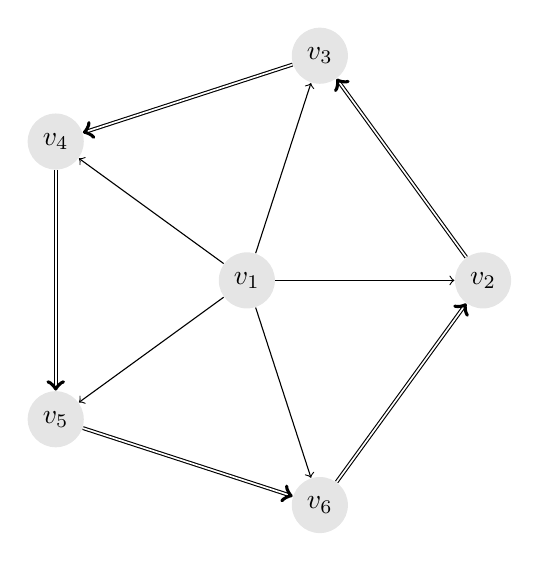
\begin{tikzpicture}
    \tikzstyle{every node} = [circle, fill=gray!20];
        \node (v1) at (0, 0)   {$v_1$};
        \node (v2) at +(0:3)   {$v_2$};
        \node (v3) at +(72:3)  {$v_3$};
        \node (v4) at +(144:3) {$v_4$};
        \node (v5) at +(216:3) {$v_5$};
        \node (v6) at +(288:3) {$v_6$};
    \foreach \n in {v2, v3, v4, v5, v6}
        \path[draw, ->] (v1) -- (\n);
\foreach \p/\n in {v2/v3, v3/v4, v4/v5, v5/v6, v6/v2}
    \path[draw, ->, double] (\p) -- (\n);
\end{tikzpicture}
\end{document}